\subsection{LRB-D under Depolarizing Noise}
\label{sub:simulation_results}

We validated the LRB-D protocol using the \texttt{sdim} qudit
stabilizer simulator \cite{sdim} for the folded $[[5,1,2]]_3$ qutrit
surface-code under the circuit-level
depolarizing noise model of \autoref{subsub:depol_model}, with the
channels inserted at the locations displayed in
\autoref{fig:lrb_d_full}. For each physical noise
strength $p$ (18 values in the sweep) and each logical depth $m$, we
(i) prepare $\ket{\bar{+}}$, (ii) apply a random length-$m$ logical
Clifford sequence followed by its ideal inverse, (iii) perform
stabilizer checks according to a chosen post-selection schedule, and
(iv) measure the logical $\bar{X}$ observable, retaining only shots
with trivial syndrome on every check. As post-selection can
drive the acceptance probability to near-zero at large $p$ and/or
large $m$, we used $10^6$ shots per depth to keep the accepted-shot
statistics usable across the sweep.

\subsubsection{Terminal post-selection: strong non-Markovianity}
In the terminal post-selection regime, stabilizer
verification is performed only once, at the end of the sequence. This
maximizes yield, but it also allows the state to leak into (and
return from) non-trivial syndrome sectors many times before the final
filter is applied. As a consequence, the observed survival curves are
not well-described by a single-exponential decay: the LRB-D traces
exhibit behaviour that cannot be captured by the decay model of
Eq.~\eqref{eq:fseq}.


This is precisely the regime where the representation-theoretic
picture of \autoref{sub:irreps} becomes operational. As the
logical Clifford action on $\mathcal{B}(\mathcal{H}_{phys})$ contains
large multiplicities (e.g., $m_{triv}=201$ and $m_{pauli}=2241$), the
twirled effective channel has many decay eigenmodes available in the
stabilizer-relevant subspace. Terminal post-selection does not
suppress these modes; instead, it produces a depth-dependent mixture
of them through repeated excursions into the syndrome sectors,
yielding the non-Markovian curves in \autoref{fig:sim_terminal_nofit}.
In this regime it is therefore difficult to assign a single,
protocol-independent logical gate fidelity to the device, since
the extracted decay rate depends sensitively on which portion of the
curve is fit.

\begin{figure}[H]
  \centering
  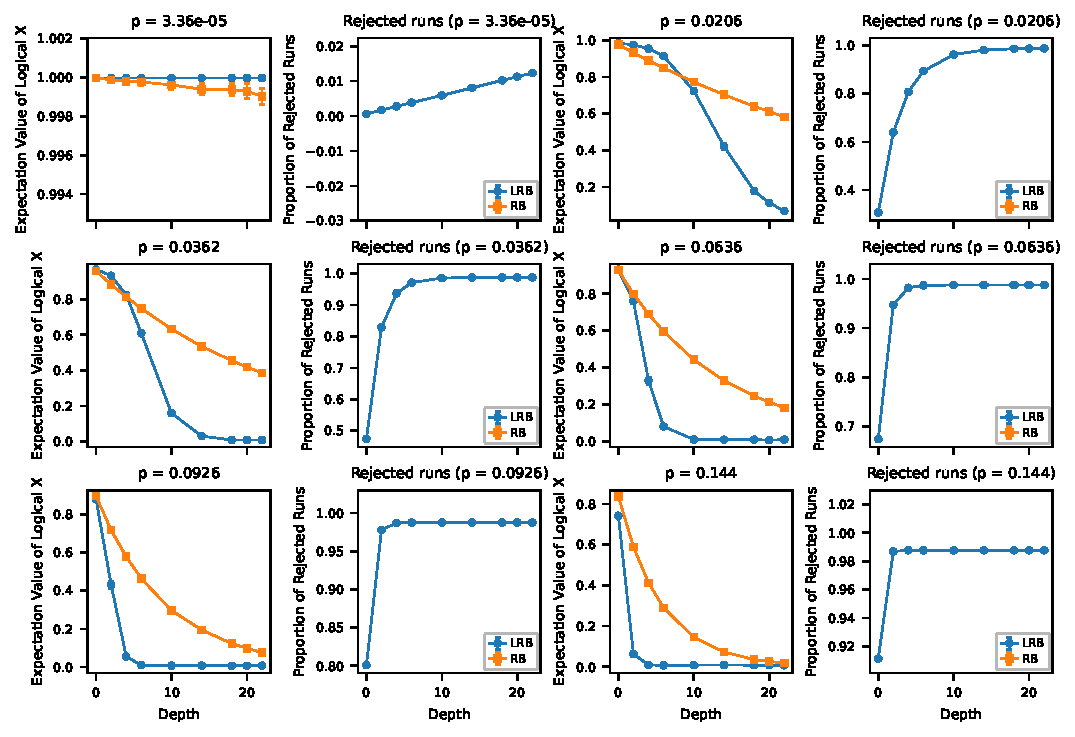
\includegraphics[width=0.95\textwidth]{
    figures/const-0-Summary-Graph-NoFit.pdf}
  \caption{Terminal post-selection. We pick out 6 $p$ values that display the non-Markovian evolution of the LRB-D traces. Columns 1 and 3: $\langle \bar{X}\rangle$ versus logical depth for
    LRB-D (blue) compared to a $\langle {X}\rangle$ versus physical RB baseline (orange). Columns 2 and 4: fraction of rejected shots versus depth. The LRB-D traces
    are visibly non-exponential, consistent with depth-dependent
    mixing among many decay modes when stabilizer filtering is applied
    only at the end of the sequence.}
  \label{fig:sim_terminal_nofit}
\end{figure}

\subsubsection{Uniform-interval post-selection: interpolating between
Markovian and non-Markovian regimes}
We next perform uniform-interval post-selection,
where stabilizers are checked every $k$ logical Cliffords and the run
is rejected as soon as a non-trivial syndrome is detected. This
introduces an adjustable reset timescale for the syndrome degrees
of freedom. All fitting in this subsection is confined to these
interval-check runs. The accepted-shot survival curves are fit to the
decay model of Eq.~\eqref{eq:fseq} with the offset fixed to $B = 0$,
since a fully depolarized logical qutrit yields a vanishing $\bar{X}$
expectation, and fidelities are extracted through Eq.~\eqref{eq:fbar}.

\paragraph{Near-Markovian limit ($k=1$).}
For $k=1$, the code-space projector is effectively applied after
every logical gate. Empirically, this recovers decay curves that are
well-approximated by a single exponential, as seen in
\autoref{fig:sim_unif1_fit}. Conceptually, frequent projection
suppresses the buildup of syndrome memory and collapses the dynamics
toward the minimal two-eigenvalue structure familiar from single-qutrit
RB (a trivial mode and a Pauli mode), in sharp contrast to the
high-multiplicity structure discussed in \autoref{sub:irreps}.

\begin{figure}[H]
  \centering
  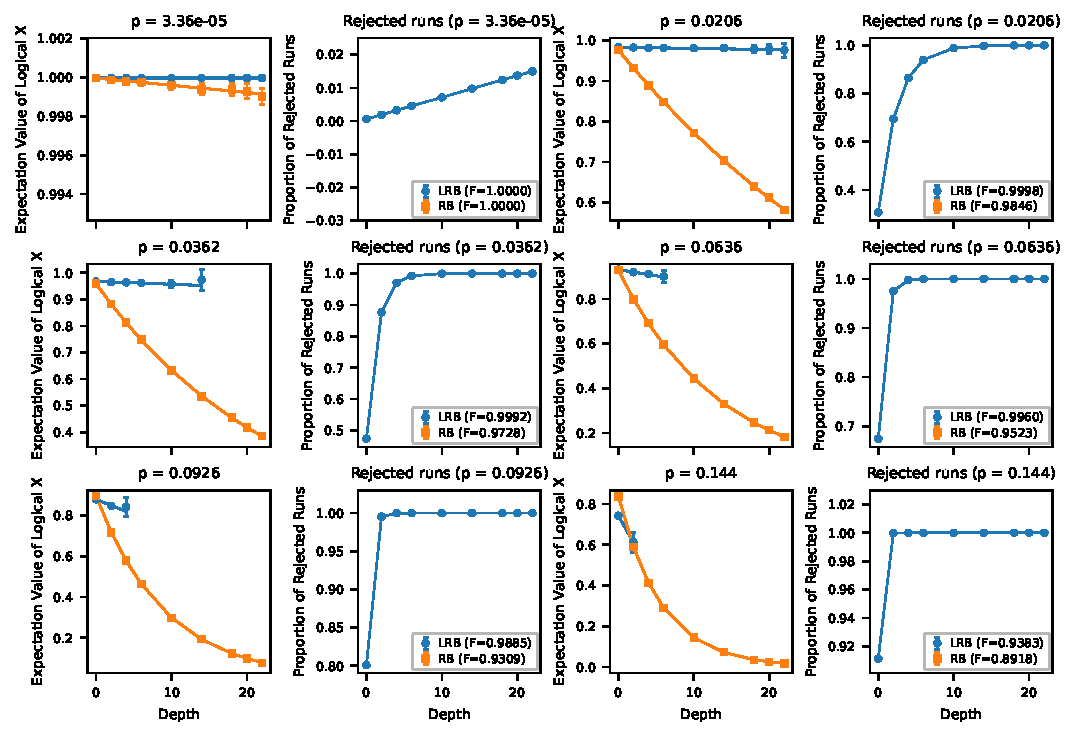
\includegraphics[width=0.95\textwidth]{
    figures/unif-1-Summary-Graph-Fit.pdf}
  \caption{Uniform interval $k=1$.
    Frequent stabilizer filtering largely restores a single-exponential
    decay model for LRB-D, at the expense of rapidly
    increasing rejection with $p$ and $m$. The \texttt{F} in the legend represents the average (logical) gate fidelity, and we notice that we get a significant improvement in fidelity due to the encoding.}
  \label{fig:sim_unif1_fit}
\end{figure}

\paragraph{Intermediate intervals ($k=2,3,4$).}
Observing \autoref{fig:sim_unif2_fit}, \autoref{fig:sim_unif3_fit}, and \autoref{fig:sim_unif4_fit}, for $k=2,3,4$, we still obtain usable single-exponential
approximations across much of the sweep, but
small deviations become more apparent as $k$ increases. Interpreted
through \autoref{sub:irreps}, these deviations reflect the gradual
reintroduction of additional decay modes associated with the many
copies of $V_{triv}$ and $V_{pauli}$ that become accessible within
each $k$-gate window. In other words, uniform-interval post-selection
interpolates between the two-mode RB-like limit ($k=1$) and the
strongly multi-mode terminal limit.

\begin{figure}[H]
  \centering
  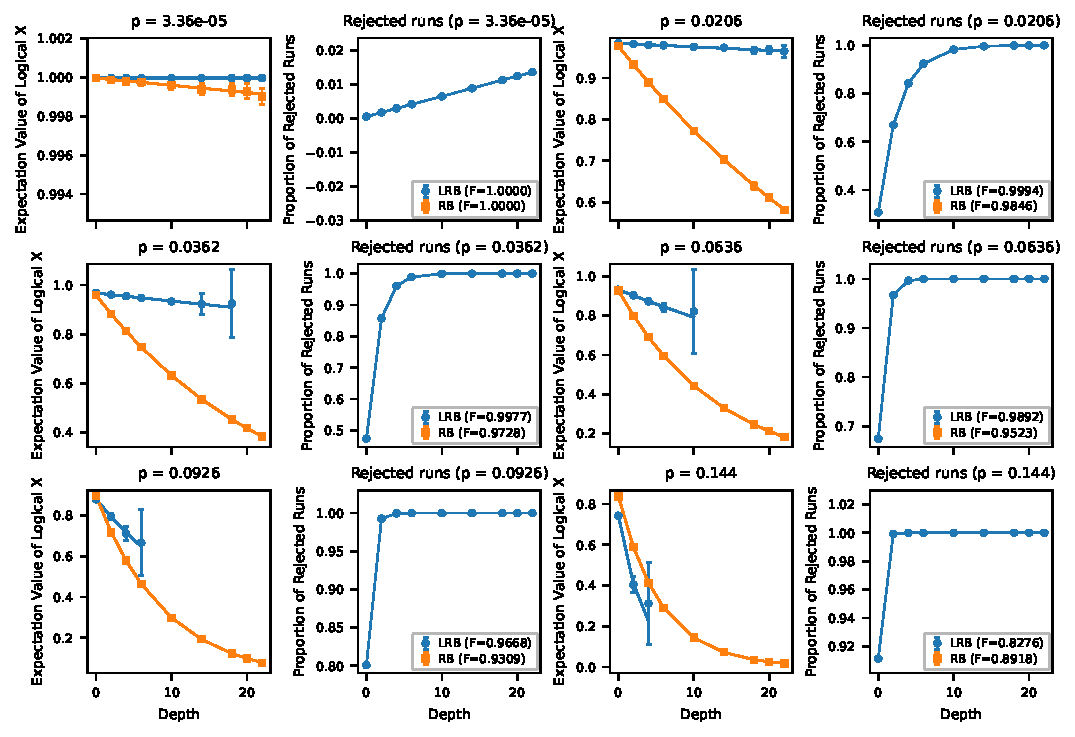
\includegraphics[width=0.95\textwidth]{
    figures/unif-2-Summary-Graph-Fit.pdf}
  \caption{Uniform interval $k=2$.
    Single-exponential fits remain a good approximation, but the
    extracted decay begins to show mild contamination from additional
    modes permitted between checks.}
  \label{fig:sim_unif2_fit}
\end{figure}

\begin{figure}[H]
  \centering
  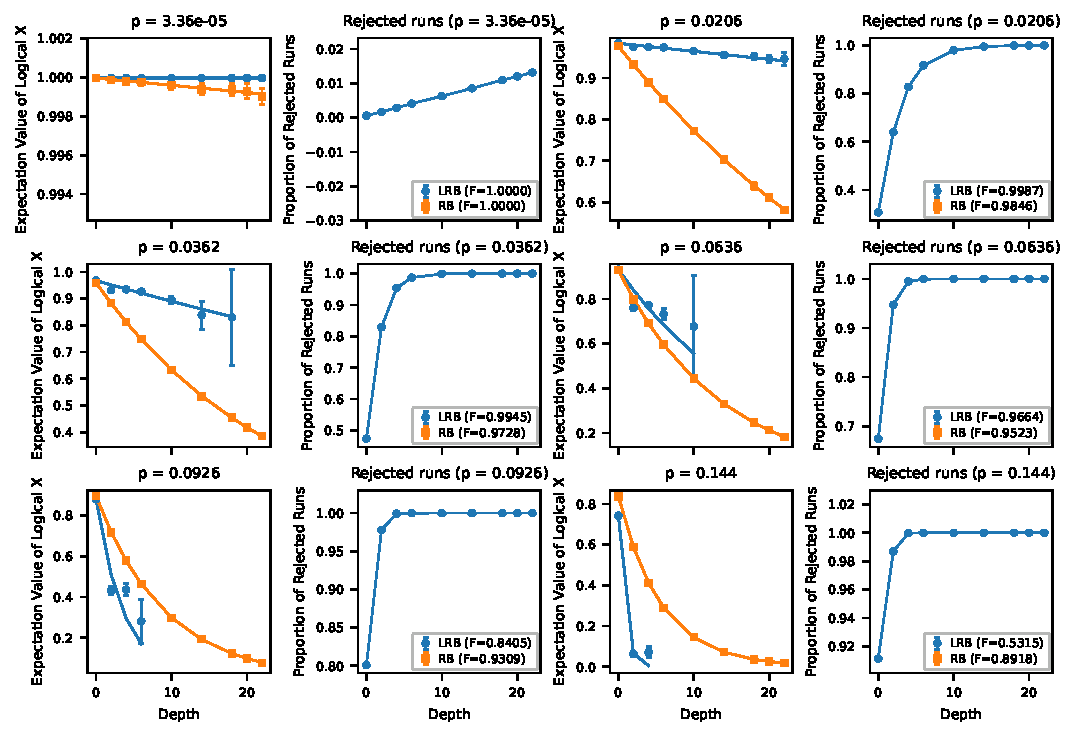
\includegraphics[width=0.95\textwidth]{
    figures/unif-3-Summary-Graph-Fit.pdf}
  \caption{Uniform interval $k=3$.
    Increasing the time between projections further increases the
    influence of syndrome-sector dynamics and amplifies departures
    from a pure single-mode decay.}
  \label{fig:sim_unif3_fit}
\end{figure}

\begin{figure}[H]
  \centering
  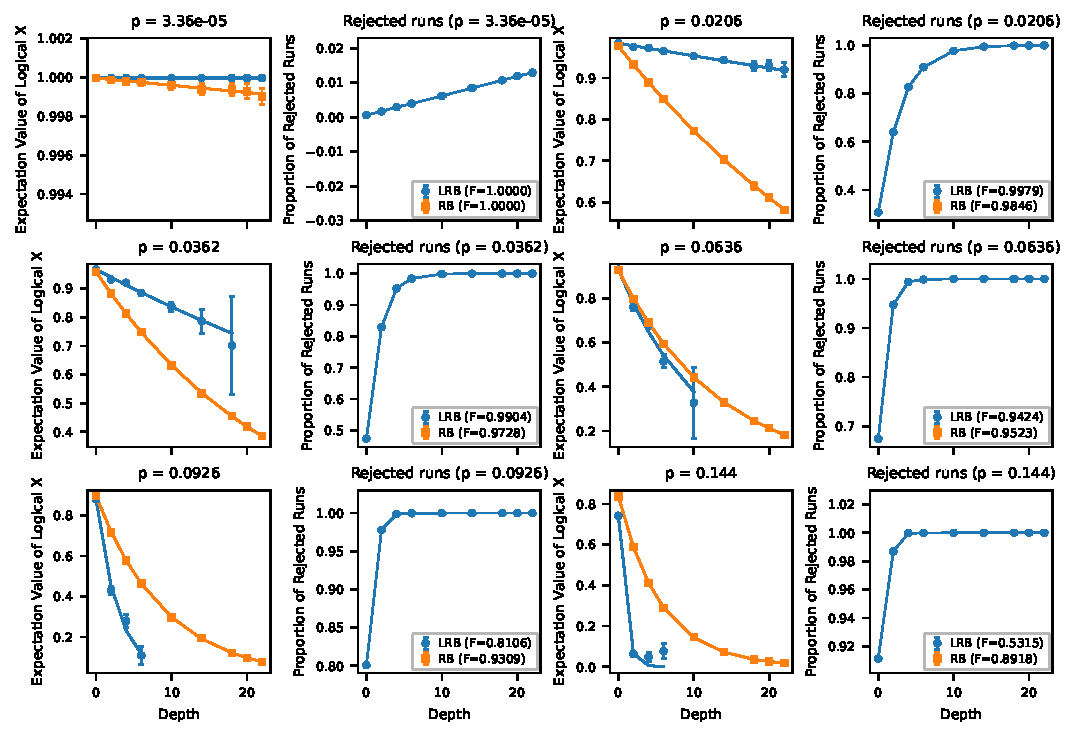
\includegraphics[width=0.95\textwidth]{
    figures/unif-4-Summary-Graph-Fit.pdf}
  \caption{Uniform interval $k=4$.
    A practical compromise regime: yields improve relative to $k=1$
    while remaining close enough to exponential behavior to extract an
    effective decay rate in much of the sweep.}
  \label{fig:sim_unif4_fit}
\end{figure}

\paragraph{Extreme intervals: re-emergent non-Markovianity.}
At large check intervals, the LRB-D curves become visibly more
irregular and less amenable to a single-exponential description.
\autoref{fig:sim_unif22_fit} shows an extreme example
(\texttt{$k=11$}), where the fitted curve captures only an average
trend while the data exhibit clear multi-timescale structure,
reflecting increased mixing among the many irrep-associated eigenmodes
between stabilizer projections. More generally, when $k$
becomes large, it no longer makes sense to interpret the LRB-D trace
through a single Markovian exponential decay model. The post-selected
(acceptance-conditioned) dynamics within the code manifold can mix
multiple irrep-associated decay modes \emph{in a depth-dependent way}
over each interval, so enforcing a fit to Eq.~\eqref{eq:fseq} becomes
a coarse phenomenological summary rather than a meaningful logical
fidelity estimator. In our folded-code sweeps, we observe that beyond about
$k=4$ the curves become strongly non-exponential across a substantial
portion of the parameter range, with visibly increasing non-Markovian
structure. For this reason, we focus our quantitative fitting and
pseudo-threshold extraction on $k=1$ through $k=4$,
using larger $k$ primarily to illustrate the non-Markovian crossover.

\begin{figure}[H]
  \centering
  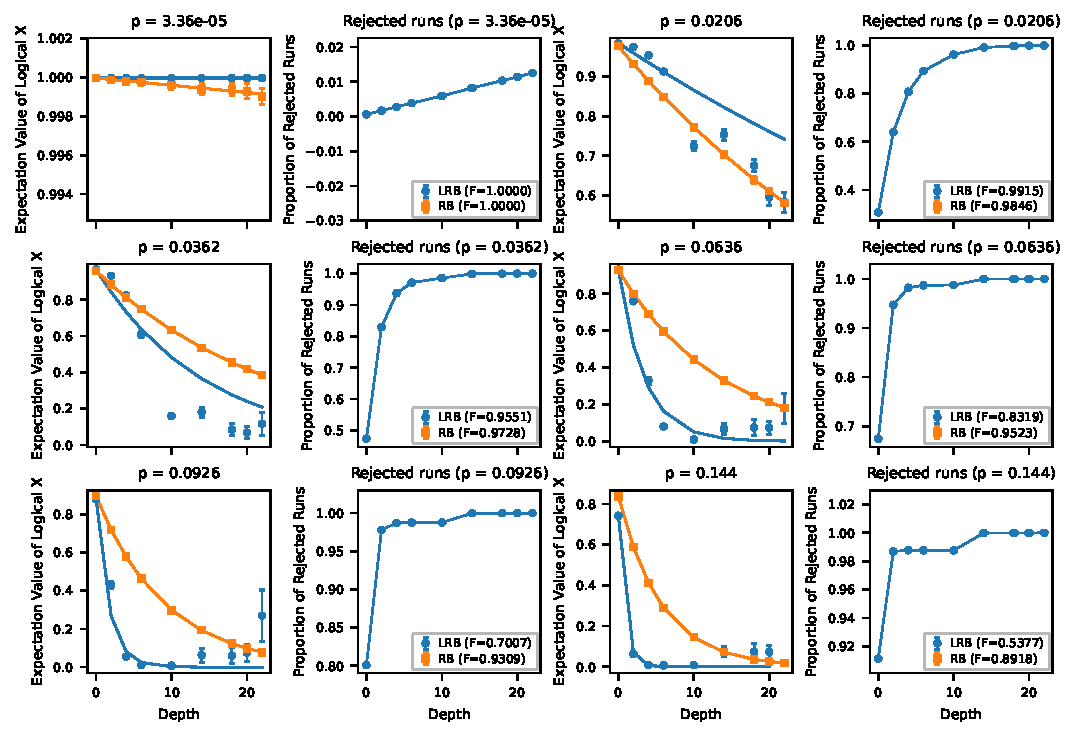
\includegraphics[width=0.95\textwidth]{
    figures/unif-11-Summary-Graph-Fit.pdf}
  \caption{Extreme uniform interval $k=11$.
    With rare stabilizer filtering throughout a logical Clifford sequence, the syndrome bath has time to
    develop substantial memory, and non-Markovian features re-emerge
    even under uniform interval post-selection.}
  \label{fig:sim_unif22_fit}
\end{figure}

\subsubsection{Pseudo-threshold analysis and the cost of post-selection}
In \autoref{fig:pseudo_threshold_panels}, we restrict the
pseudo-threshold analysis to $k=1$ through $k=4$.
To quantify when LRB-D provides an advantage over an unencoded
physical baseline, we compare the extracted error rates from (i)
LRB-D under uniform $k$-interval post-selection and (ii) standard
single-qutrit RB under the same physical noise parameter $p$. For each
$k$, we define a \emph{pseudo-threshold} $p^\star(k)$ as the value of
$p$ where the fitted LRB-D error rate intersects the fitted RB error
rate. Below $p^\star(k)$, the post-selected logical protocol exhibits
lower error than the physical reference. Above $p^\star(k)$, the
benefits of encoding are outweighed by the accumulated error paths
and the severe acceptance loss.

\begin{figure}[H]
  \centering
  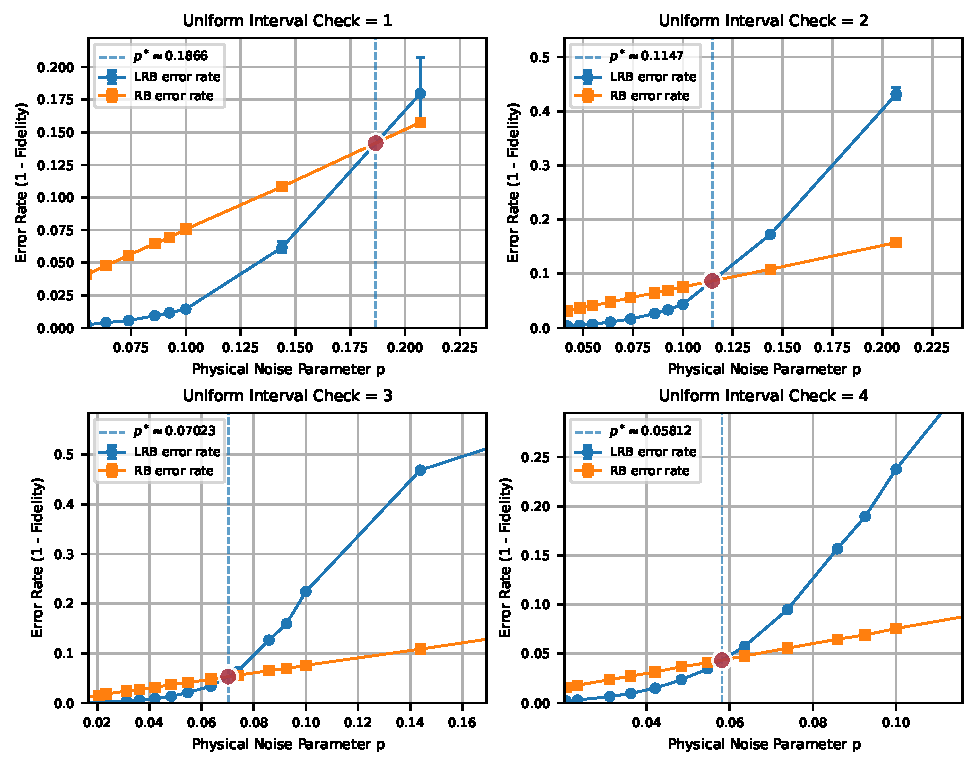
\includegraphics[width=\textwidth]{figures/unif-threshold-error-vs-p-paper-grid.pdf}
  \caption{Pseudo-threshold construction for uniform-interval post-selection.
    We plot fitted RB and LRB-D error rates versus $p$ for uniform check intervals
    $k=1,2,3,4$ and define $p^\star(k)$ by their intersection. As we get more liberal with our intervals, we observe that the pseudo-threshold starts to drop. However, the tradeoff is that we have more shot acceptances at each error parameter $p$.}
  \label{fig:pseudo_threshold_panels}
\end{figure}

For the folded $[[5,1,2]]_3$ patch, we find
$p^\star(1)\approx 0.186611 \pm 0.012320$,
$p^\star(2)\approx 0.114679 \pm 0.000768$,
$p^\star(3)\approx 0.070231 \pm 0.000258$,
and $p^\star(4)\approx 0.058116 \pm 0.000202$.
\autoref{fig:pseudo_threshold_trend} summarizes the decline
of $p^\star(k)$ with increasing $k$, quantifying the intuitive and
irrep-consistent statement that allowing longer syndrome sector
correlation times degrades the effective logical protection.

\begin{figure}[H]
  \centering
  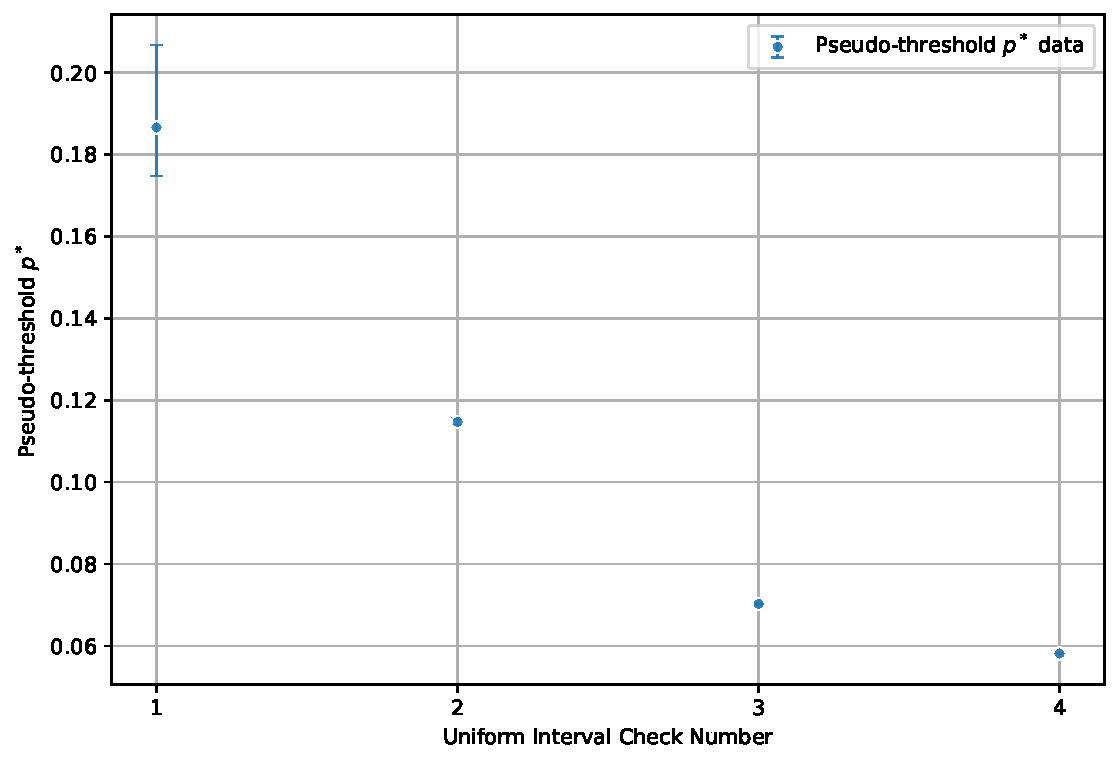
\includegraphics[width=0.65\textwidth]{
    figures/unif-1-to-4-pseudo-threshold-vs-interval-check-fit.pdf}
  \caption{Pseudo-threshold versus check interval. The
    pseudo-threshold decreases rapidly as stabilizer checks become less
    frequent, reflecting increased multi-mode contamination and
    longer-lived syndrome memory between projections to the codespace.}
  \label{fig:pseudo_threshold_trend}
\end{figure}

Post-selection is essential here because $[[5,1,2]]_3$ is an error-\emph{detection} code: it allows us to benchmark a small early-FTQC patch
without committing to an ambiguous decoder and violating Knill-Laflamme's error correction conditions. It also provides a tunable
knob ($k$) that cleanly exposes the crossover from RB-like (two-mode)
exponential decay to multi-mode, non-Markovian behavior described in
\autoref{sub:irreps}. 

The principal drawback is sampling overhead: as
seen in the rejection panels of \autoref{fig:sim_unif1_fit}--
\autoref{fig:sim_unif22_fit}, the accepted fraction can collapse
quickly with $p$ and depth, requiring very large shot counts to
maintain statistical power. Moreover, because LRB-D reports a
\emph{conditional} logical performance (conditioned on no detected
error), it does not directly represent the unconditional reliability
of a long computation. Instead, it characterizes the quality of the
logical dynamics within the detected code manifold and how strongly
they are perturbed by excursions into syndrome sectors.